\documentclass[12pt,letterpaper]{article}

\usepackage{fullpage}
\usepackage[top=2cm, bottom=4.5cm, left=2.5cm, right=2.5cm]{geometry}
\usepackage{amsmath,amsthm,amsfonts,amssymb,amscd}
\usepackage{lastpage}
\usepackage{enumitem}
\usepackage{fancyhdr}
\usepackage{mathrsfs}
\usepackage{xcolor}
\usepackage{graphicx}
\usepackage{listings}
\usepackage[colorlinks=true]{hyperref}
\usepackage{bookmark}
\usepackage{listing}
\usepackage{siunitx}
%\usepackage{appendix}
\usepackage{xcolor}
\usepackage{siunitx}
\usepackage{microtype}
\usepackage{float}
\usepackage{titling}
\usepackage{svg}
\usepackage{longtable}
\usepackage[title,titletoc]{appendix}
\usepackage[UKenglish]{isodate}
\usepackage{derivative}
\usepackage{physics}
\usepackage{cancel}
\usepackage{empheq}
\usepackage{draftwatermark}

\SetWatermarkAngle{45}
\SetWatermarkScale{1.75}
\SetWatermarkColor{red!15}
\SetWatermarkFontSize{42pt}
\SetWatermarkText{\shortstack{\bfseries\sffamily DRAFT! \\ [1em] \bfseries\sffamily DRAFT! \\ [1em ]\bfseries\sffamily DRAFT! }}

\definecolor{codegreen}{rgb}{0,0.6,0}
\definecolor{codegray}{rgb}{0.5,0.5,0.5}
\definecolor{codepurple}{rgb}{0.58,0,0.82}
\definecolor{backcolour}{rgb}{0.95,0.95,0.92}

\lstdefinestyle{mystyle}{
	backgroundcolor=\color{backcolour},   
	commentstyle=\color{codegreen},
	keywordstyle=\color{magenta},
	numberstyle=\tiny\color{codegray},
	stringstyle=\color{codepurple},
	basicstyle=\ttfamily\footnotesize,
	breakatwhitespace=false,         
	breaklines=true,                 
	captionpos=b,                    
	keepspaces=true,                 
	numbers=left,                    
	numbersep=5pt,                  
	showspaces=false,                
	showstringspaces=false,
	showtabs=false,                  
	tabsize=2
}

\cleanlookdateon% Remove ordinal day reference
\lstset{style=mystyle}
\setlength{\parindent}{0.0in}
\setlength{\parskip}{0.05in}
\pagestyle{fancyplain}
\headheight 35pt
\rhead{\theauthor\\\today}               
\chead{\textbf{\Large Homework \homeworknumber{}}}
\lhead{\coursenumber \\ \coursename{}}
\lfoot{}
\cfoot{}
\rfoot{\small\thepage}
\headsep 1.5em
\renewcommand{\headrulewidth}{2pt}

% Edit these as appropriate
\author{Evan Burke}
\newcommand\homeworknumber{1} 
\title{Homework \homeworknumber}
\newcommand\coursenumber{AEE 553}
\newcommand\coursename{Compressible Flow}
\newcommand\instructor{Dr. Carson Running}
\newcommand\studentID{101318838}   
     
%\newcommand\Name{\author}                

\begin{document}
	\graphicspath{{../images}}
	\begin{titlepage}
	\newcommand{\HRule}{\rule{\linewidth}{0.5mm}}
	
	\begin{figure}
		\centering
		\includesvg[scale=0.85]{images/University_of_Dayton}\\[1cm]
	\end{figure}
	
	\center 
	\quad\\[1.5cm]
	\textsl{\Large \coursenumber\ \textemdash\ \coursename}\\[0.5cm] 
	\textsl{\large Department of Mechanical and Aerospace Engineering}\\[0.5cm] 
	\makeatletter
	\HRule \\[0.4cm]
	{ \huge \bfseries \@title}\\[0.4cm] 
	\HRule \\[1.5cm]
	\begin{minipage}{0.4\textwidth}
		\begin{flushleft} \large
			\emph{Author:}\\
			\@author 
		\end{flushleft}
	\end{minipage}
	~
	\begin{minipage}{0.4\textwidth}
		\begin{flushright} \large
			\emph{Instructor:} \\
			\textup{\instructor}
		\end{flushright}
	\end{minipage}\\[3cm]
	\makeatother
	%{\large An Assignment submitted for the UoS:}\\[0.5cm]
	%{\large \emph{Place Your Course Code and Course Name Here}}\\[0.5cm]
	\vfill
	{\large \today}\\[2cm]
	\vfill 
\end{titlepage}
	
	\tableofcontents
	
	%    \maketitle
	
	%\thispagestyle{empty}
	\newpage
	
	\section*{Nomenclature}
	
	{\renewcommand\arraystretch{1.0}
		\noindent\begin{longtable}{@{}l @{\quad=\quad} l@{}}
			$A$  & amplitude of oscillation \\
			$a$ &    cylinder diameter \\
			$C_p$& pressure coefficient \\
			$Cx$ & force coefficient in the \textit{x} direction \\
			$Cy$ & force coefficient in the \textit{y} direction \\
			c   & chord \\
			d$t$ & time step \\
			$Fx$ & $X$ component of the resultant pressure force acting on the vehicle \\
			$Fy$ & $Y$ component of the resultant pressure force acting on the vehicle \\
			$f, g$   & generic functions \\
			$h$  & height \\
			$i$  & time index during navigation \\
			$j$  & waypoint index \\
			$K$  & trailing-edge (TE) nondimensional angular deflection rate
	\end{longtable}}
	
	\addcontentsline{toc}{section}{Nomenclature}
	\newpage
	
	\section*{Problem 1}
	In an inviscid flow, a small change in pressure d$p$, is related to a small change in velocity, d$u$, by

	\begin{equation*}
		\dd p = - \rho u\dd u\,,
	\end{equation*}
	
	which is referred to as Euler’s equation and is derived from the conservation of momentum.
	\addcontentsline{toc}{section}{Problem 1}
	
	\begin{enumerate}[label=(\alph*)]
		\label{Sec:Problem1}
		\item Using this relation, derive a differential relation for the fractional density change $\dd \rho / \rho$ as a function of the fractional change in velocity $\dd u/ u$, with the fluid's compressibility $\tau$ as a coefficient.
		\addcontentsline{toc}{subsection}{(a)}
		
		\medskip
		
		\begin{enumerate}[label=\arabic*.]
			
			\item{\textbf{Givens}} \\
				Euler's Equation\\
				$\dd \rho / \rho $ \\
				$\dd u / u$ \\
				$\tau = \frac{1}{\rho} \frac{\dd \rho}{\dd p}$
				\addcontentsline{toc}{subsubsection}{Givens}

			\item{\textbf{Assumptions}} \\
			Inviscid flow, small changes in pressure and velocity.\\
			\addcontentsline{toc}{subsubsection}{Assumptions}
			
			
			\item{\textbf{Solution}} \\
				Given the definition of compressibility,
			
			
			\begin{equation*}
				\tau = \frac{1}{\rho} \frac{\dd \rho}{\dd p} \,,
			\end{equation*}
			
			we can solve algebraically for an expression defining $\dd p$ in terms of $\tau$ and the fractional change in density, $\dd \rho / \rho$:
			
			\begin{equation*}
				\dd p = \frac{1}{\tau} \frac{\dd \rho}{\rho}
			\end{equation*}
		
			Setting the LHS of this new equation equal to the RHS of Euler's equation and solving for $\dd \rho / \rho$:
			
			\begin{equation*}
				\frac{1}{\tau} \frac{\dd \rho}{\rho} = - \rho u\dd u\
			\end{equation*}
			
			
			
			\begin{equation*}
				\frac{\dd \rho}{\rho} = - \rho \tau u \dd u
			\end{equation*}
			
			Finally, we can express this equation in terms of the fractional change in velocity, $\dd u / u$, by multiplying the RHS by $u / u$:
			
			\begin{equation*}
					\boxed{\frac{\dd \rho}{\rho} = - \rho \tau u^2 \frac{\dd u}{u}}
			\end{equation*} 
			\addcontentsline{toc}{subsubsection}{Solution}

		\end{enumerate}
		
		\item Show that $\tau$ for isentropic flows simplifies to
		\addcontentsline{toc}{subsection}{(b)}
		
			\begin{equation*}
				\tau = \frac{1}{\gamma p} \,.
			\end{equation*}
	
			\begin{enumerate}[label=\arabic*.]
	
				\item{\textbf{Givens}} \\
					\begin{equation*}
						\tau = \frac{1}{\rho} \frac{\dd \rho}{\dd p}
					\end{equation*}
					\addcontentsline{toc}{subsubsection}{Givens}


				\item{\textbf{Assumptions}} \\
					Isentropic flow (therefore, adiabatic and reversible). Thermally perfect gas (TPG).
					\addcontentsline{toc}{subsubsection}{Assumptions}


				\item{\textbf{Solution}} \\
					The 1\textsuperscript{st} law of thermodynamics indicates that for a closed system containing a constant mass the specific internal energy can be defined as
					
					\begin{equation*}
						\dd e = \delta q + \delta w\,,
					\end{equation*}

					where $\delta q$ and $\delta w$ are the amount of heat entering the system and work being done on the system, respectively. To be considered isentropic, a system must be both adiabatic and reversible.\\
					\medskip
					\\
					An adiabatic system is one where there is no heat transfer in or out of the system. Represented mathematically, the first law for an adiabatic system can be written as:

					\begin{equation*}
						\dd e = \delta w.
					\end{equation*}
					
					A reversible system is one where there are no dissipative phenomena present in the system (shear forces, mass diffusion, etc.). Represented mathematically, the first law for a reversible system can be written as:
					
					\begin{equation*}
						\dd e = \delta q - p\dd \nu\,,
					\end{equation*}			
						
					where $-p\dd \nu$ represents reversible flow work. \\
					
					The 1\textsuperscript{st} law for isentropic process, by definition both adiabatic and reversible, can be expressed as:
					\begin{equation*}
						\dd e = -p\dd \nu
					\end{equation*}
					\medskip
					\\
					
					The 2\textsuperscript{nd} law of thermodynamics tells us the direction that a process will occur. To discuss the 2\textsuperscript{nd} law, we evaluate the change in specific entropy,
					
					\begin{equation*}
						\dd s = \frac{\delta q}{T} + \delta s_{irreversible}\,,
					\end{equation*}
				
					
					where $\delta s_{irreversible}$ represents lost or unrecoverable energy and is always $\ge$ 0. Combining this definition of specific entropy with our 1\textsuperscript{st} law representations of adiabatic processes, we obtain the following for adiabatic processes:
					
					\begin{equation*}
						\dd s = \dd s_{irreversible}
					\end{equation*}
					
					\begin{equation*}
						\dd s \ge 0
					\end{equation*}
					
					For a reversible process, $\delta s_{irreversible}$ must, by definition, equal 0. Therefore, combining the 1\textsuperscript{st} and 2\textsuperscript{nd} law produces the following:
					
					\begin{equation*}
						\dd s = \frac{\delta q}{T}
					\end{equation*}
					
					We have now defined both adiabatic and reversible processes according to the 1\textsuperscript{st} and 2\textsuperscript{nd} laws of thermodynamics. We can now revisit the definition of entropy and evaluate the implications of a system being both adiabatic and reversible.
					
					\begin{equation*}
						\dd s = \delta q + \delta s_{irreversible}
					\end{equation*}
				
					\begin{equation*}
						\dd s = \cancelto{0, \mathrm{adiabatic}}{\delta q} + \cancelto{0, \mathrm{reversible}}{\delta s_{irreversible}}				
					\end{equation*}
					
					\begin{equation*}
						\boxed{\dd s = 0}
					\end{equation*}
				
					A system that is both adiabatic and reversible must also be isentropic. With this understanding, the definition of compressibility, $\tau$, can be revisited.
				
					\begin{equation*}
						\tau = \frac{1}{\rho}\frac{\dd \rho}{\dd p} = - \frac{1}{\nu}\frac{\dd\nu}{\dd p}
					\end{equation*}
				
					Recall the isentropic 1\textsuperscript{st} law representation of the change in specific internal energy, $\dd e$:
					
					\begin{equation*}
						\dd e = - p \dd \nu
					\end{equation*}
				
					Assuming the working fluid to be a thermally perfect gas, this can be expressed as:
					
					\begin{equation*}
						c_\nu \dd T= -p \dd \nu
					\end{equation*}
					
					\begin{equation*}
						\boxed{\dd \nu = - \frac{c_{\nu}\dd T}{p}}
					\end{equation*}				
				
					Now, recall the definition of enthalpy:
					
					\begin{equation*}
						h = e + p\nu
					\end{equation*}
					
					Taking the exact differential leads to:
					
					\begin{equation*}
						\dd h = \dd e + p\dd \nu + \nu \dd p
					\end{equation*}
					
					Replacing $\dd e$ with its isentropic 1\textsuperscript{st} law representation:
						
					\begin{equation*}
						\dd h = -p\dd \nu + p\dd\nu + \nu \dd p
					\end{equation*}
					\begin{equation*}
						\dd h = \nu \dd p
					\end{equation*}
				
					Assuming the working fluid to be a thermally perfect gas, $\dd h$ can be expressed as:
					
					\begin{equation*}
						\dd h = c_p \dd T
					\end{equation*}
					
					Therefore:
					
					\begin{equation*}
						\boxed{\nu \dd p = c_p \dd T}
					\end{equation*}
				
				
					Plugging the boxed expressions back in to our original expression for $\tau$: 
					
					\begin{equation*}
						\tau = - \frac{1}{\left(c_{p}\dd T\right)} \left(-\frac{c_{\nu}\dd T}{p}\right)
					\end{equation*}
					\begin{equation*}
						\tau = \frac{c_{\nu}}{c_p}\frac{1}{p}
					\end{equation*}
					The ratio of specific heats, $\gamma$, is defined as
					\begin{equation*}
						\gamma = \frac{c_p}{c_{\nu}}\,,
					\end{equation*}
					and can be substituted into the previous equation to arrive at the final result:
					\begin{equation*}
						\boxed{\tau = \frac{1}{\gamma p}}
					\end{equation*}
					\addcontentsline{toc}{subsubsection}{Solution}		

			\end{enumerate}

		\item The velocity at a point in an isentropic flow of air is u = 63 m/s traveling by a Cessna
		172 prop aircraft. The density and pressure are 1.23 kg/m\textsuperscript{3} and 1.01 $\times$ 10\textsuperscript{5} Pa, respectively.
		If the fractional velocity change is 0.01, what is the fractional density change? Do not look
		up a value for $\tau_{air}$. Instead, use your result from part (b). $\gamma$ = 1.4 for air.
		\addcontentsline{toc}{subsection}{(c)}
		
		\begin{enumerate}[label=\arabic*.]
			
			\item{\textbf{Givens}} \\
			$u = 63 \ \mathrm{m/s}$\\
			$\rho = 1.23 \ \mathrm{kg/m\textsuperscript{3}}$\\
			$p = 1.01 \times 10^5 \  \mathrm{Pa}$\\
			$\frac{\dd u}{u} = 0.01$\\
			$\gamma_{air} = 1.4$\\		
			\addcontentsline{toc}{subsubsection}{Givens}


			\item{\textbf{Assumptions}} \\
			Isentropic flow, $\tau_{air} = \frac{1}{\gamma p}$.
			\addcontentsline{toc}{subsubsection}{Assumptions}


			\item{\textbf{Solution}} \\
			
			From part (a), the fractional density change can be expressed as:
			\begin{equation*}
				\frac{\dd \rho}{\rho} = - \rho \tau u^2 \frac{\dd u}{u}
			\end{equation*}
		
			Using the result from part (b), we can express the fractional density change in terms of $\gamma$ and $p$:
			
			\begin{equation*}
				\frac{\dd \rho}{\rho} = - \rho \left( \frac{1}{\gamma p} \right) u^2 \frac{\dd u}{u}
			\end{equation*}
			
			From the problem statement, we now have all of the givens required to solve for $\dd \rho / \rho$:
			
			\begin{equation*}
				\frac{\dd \rho}{\rho} = - \left(1.23\left[\frac{kg}{m^3}\right]\right) \left(\frac{1}{1.4}\right)\left(\frac{1}{1.01 \times 10^5}\left[\frac{N}{m^2}\right]^{-1} \right) \left(63 \left[\frac{m}{s}\right]\right)^2 \left(0.01\right)
			\end{equation*}

			Performing dimensional analysis to confirm validity of equation:
			
			\begin{equation*}
				\left[\frac{kg}{m^3}\right] \times \left[\frac{m^2}{N}\right] \times \left[\frac{m^2}{s^2}\right] \rightarrowtail \left[\frac{kg \cdot m}{s^2}\right] \times \left[\frac{1}{N}\right] \rightarrowtail \cancelto{1}{\left[\frac{N}{N}\right]} \checkmark
			\end{equation*}

			\begin{equation*}
				\boxed{\frac{\dd \rho}{\rho} = -0.03\%}
			\end{equation*}
			
			All calculations were performed in Python, see Appendix \ref{Problem1Python} for relevant code. 

			\addcontentsline{toc}{subsubsection}{Solution}		

		\end{enumerate}

		\item Repeat part (c) for a local velocity $u$ = 980 m/s, representative of an SR-71 Blackbird. Allow the fractional velocity change to still be 0.01. You may still assume isentropic flow. 
		\addcontentsline{toc}{subsection}{(d)}
		
		\begin{enumerate}[label=\arabic*.]
			
			\item{\textbf{Givens}} \\
			$u = 980 \ \textrm{m/s}$\\
			$\rho = 1.23 \ \mathrm{kg/m\textsuperscript{3}}$\\
			$p = 1.01 \times 10^5 \  \mathrm{Pa}$\\
			$\frac{\dd u}{u} = 0.01$\\
			$\gamma_{air} = 1.4$\\
			\addcontentsline{toc}{subsubsection}{Givens}

			
			\item{\textbf{Assumptions}} \\
			Isentropic flow, $\tau_{air} = \frac{1}{\gamma p}$.
			\addcontentsline{toc}{subsubsection}{Assumptions}


			\item{\textbf{Solution}} \\
			From part (a), the fractional density change can be expressed as:
			\begin{equation*}
				\frac{\dd \rho}{\rho} = - \rho \tau u^2 \frac{\dd u}{u}
			\end{equation*}
			
			Using the result from part (b), we can express the fractional density change in terms of $\gamma$ and $p$:
			
			\begin{equation*}
				\frac{\dd \rho}{\rho} = - \rho \left( \frac{1}{\gamma p} \right) u^2 \frac{\dd u}{u}
			\end{equation*}
			
			From the problem statement, we now have all of the givens required to solve for $\dd \rho / \rho$:
			
			\begin{equation*}
				\frac{\dd \rho}{\rho} = - \left(1.23\left[\frac{kg}{m^3}\right]\right) \left(\frac{1}{1.4}\right)\left(\frac{1}{1.01 \times 10^5}\left[\frac{N}{m^2}\right]^{-1} \right) \left(980 \left[\frac{m}{s}\right]\right)^2 \left(0.01\right)
			\end{equation*}
			
			Performing dimensional analysis to confirm validity of equation:
			
			\begin{equation*}
				\left[\frac{kg}{m^3}\right] \times \left[\frac{m^2}{N}\right] \times \left[\frac{m^2}{s^2}\right] \rightarrowtail \left[\frac{kg \cdot m}{s^2}\right] \times \left[\frac{1}{N}\right] \rightarrowtail \cancelto{1}{\left[\frac{N}{N}\right]} \checkmark
			\end{equation*}
			
			\begin{equation*}
				\boxed{\frac{\dd \rho}{\rho} = -8.35\%}
			\end{equation*}

			All calculations were performed in Python, see Appendix \ref{Problem1Python} for relevant code. 

			\addcontentsline{toc}{subsubsection}{Solution}		


		\end{enumerate}	
	
		\item Comment on the order-of-magnitude differences in the fractional density change between parts (c) and (d). What causes this large difference? Are both compressible flows?
		\addcontentsline{toc}{subsection}{(e)}
		
		\begin{enumerate}[label=\arabic*.]
			
			\item{\textbf{Discussion}} \\
			The fractional density change in part (d) is $\sim$ 242 times larger than the fractional density change in part (c). Given that all other initial conditions and assumptions are identical, the primary driver of the observed difference in magnitude is the flow velocity. Despite the same fractional velocity change, the freestream velocity magnitude is the dominant factor due to the $u^2$ term in our expression for fractional density change. Taking the ratio of velocity squared $u_{d}^2/u_{c}^2$ results in the same $\sim$ 242 ratio observed when comparing fractional density changes. \\The conditions illustrated in part (c) are generally not considered to be compressible due to the extremely low fractional density change. With a rule of thumb of 5\% density change as the boundary between compressible and incompressible, the density change in part (c) is too small by far to be considered compressible. In comparison, the conditions illustrated in part (d) are easily considered compressible due to the much larger density change. The air in both cases tends to become \textit{less} dense, as illustrated by the polarity of $\dd \rho/\rho$, which is caused (generally speaking) by the increase in flow velocity the fluid experiences. 
			\addcontentsline{toc}{subsubsection}{Discussion}
		\end{enumerate}
	
		\item Use this finding to explain to a classmate why high-speed (i.e., supersonic, hypersonic) flows are inherently compressible.
		\addcontentsline{toc}{subsection}{(f)}
		
		\begin{enumerate}[label=\arabic*.]

			\item{\textbf{Discussion}} \\
			High speed flows are inherently compressible due to the magnitude of their freestream flow velocity. Relatively small changes in fractional velocity can result in significant density changes, as illustrated in parts (d) and (e). Larger changes in flow velocity as would be seen in a real-world application of an aerodynamic body in high speed flow would cause even more significant density changes than shown in part (d). As flow velocities grow larger, towards hypersonic conditions, the effect of the $u^2$ term in the fractional density change equation exerts more and more influence. Despite making relatively few assumptions about the flow (isentropic, TPG), we have arrived at a fairly simple model that demonstrates the reality of compressible flow and its sensitivity to small changes in initial conditions.
			\addcontentsline{toc}{subsubsection}{Discussion}	

		\end{enumerate}
		
		
	\end{enumerate}


	\newpage
	
	\section*{Problem 2}
	\label{Sec:Problem2}
	\addcontentsline{toc}{section}{Problem 2}
	\begin{enumerate}[label=(\alph*)]
		\item Derive the following equations for $c_p$ and $c_{\nu}$ (recall, $\gamma = c_p/c_{\nu}$).
		\addcontentsline{toc}{subsection}{(a)}
		\begin{equation*}
			c_p = \frac{\gamma R}{\gamma - 1}
		\end{equation*}
		\begin{equation*}
			c_{\nu} = \frac{R}{\gamma-1}
		\end{equation*}
		
		\begin{enumerate}[label=\arabic*.]
			\item{\textbf{Givens}}
			\addcontentsline{toc}{subsubsection}{Givens}\\
			$\gamma = \frac{c_p}{c_{\nu}}$

			\item{\textbf{Assumptions}}
			\addcontentsline{toc}{subsubsection}{Assumptions}\\
			Assume ideal gas, thermally perfect gas (TPG).
			\item{\textbf{Solution}}\\
			The specific heat at constant pressure, $c_p$, is defined as:
			\begin{equation*}
				c_p = \left(\frac{\partial h}{\partial T}\right)_p
			\end{equation*}
			The specific heat at constant volume, $c_{\nu}$ is defined as:
			\begin{equation*}
				c_{\nu} = \left(\frac{\partial e}{\partial T}\right)_{\nu}
			\end{equation*}		
			For a thermally perfect gas, (TPG) these can be expressed as:
			\begin{equation*}
				c_p = \frac{\dd h}{\dd T}
			\end{equation*}	
			\begin{equation*}
				c_{\nu} = \frac{\dd e}{\dd T}
			\end{equation*}	
			Specific enthalpy, $h$, is defined as:
			\begin{equation*}
				h = e + p\nu
			\end{equation*}
			For an ideal gas, $h$ can be expressed as a function of $T$ and $\nu$:
			\begin{equation*}
				h(T,\nu) = e(T,\nu) + p\nu
			\end{equation*}
			For a TPG, chemical reactions in the flow are neglected, and $h$ can be expressed as a function of $T$ only:
			\begin{equation*}
				h(T) = e(T) + p\nu
			\end{equation*}
			Taking the exact differential:
			\begin{equation*}
				dh = de + \dd (\frac{p}{\rho})
			\end{equation*}
			Substituting using the ideal gas law:
			\begin{equation*}
				\frac{p}{\rho} = RT
			\end{equation*}
			\begin{equation*}
				dh = de + R\dd T
			\end{equation*}
			Dividing through by $\dd T$:
			\begin{equation*}
				\left(\frac{\dd h}{\dd T}\right) = \left(\frac{\dd e}{\dd T}\right) + R
			\end{equation*}
			Recognizing that enthalpy and energy terms are in the forms of the previously defined specific heats and substituting gives us another useful equation:
			\begin{equation*}
				c_p = c_{\nu} + R
			\end{equation*}
			\begin{equation*}
				\boxed{c_p - c_{\nu} = R}
			\end{equation*}
		
			Dividing through by $c_p$:
			\begin{equation*}
				\frac{c_p}{c_p} - \frac{c_{\nu}}{c_p} = \frac{R}{c_p}
			\end{equation*}
			\begin{equation*}
				1 - \frac{c_{\nu}}{c_p} = \frac{R}{c_p}
			\end{equation*}
			Rearranging to solve for $c_p$:
			\begin{equation*}
				c_p = \frac{R}{1-\frac{c_{\nu}}{c_p}}
			\end{equation*}
			Substituting $\gamma$ into the equation and rearranging:
			\begin{equation*}
				c_p = \frac{R}{1-\frac{1}{\gamma}}
			\end{equation*}
			\begin{equation*}
				c_p = \frac{R}{\frac{\gamma-1}{\gamma}}
			\end{equation*}
			\begin{equation*}
				\boxed{c_p = \frac{\gamma R}{\gamma-1}}
			\end{equation*}
			Recall the relationship between specific heats first derived:
			\begin{equation*}
				c_p - c_{\nu} = R
			\end{equation*}
			Dividing through by $c_{\nu}$:
			\begin{equation*}
				\frac{c_p}{c_{\nu}} - \frac{c_{\nu}}{c_\nu} = \frac{R}{c_\nu}
			\end{equation*}
			Simplify and rearrange:
			\begin{equation*}
				\gamma - 1 = \frac{R}{c_\nu}
			\end{equation*}
			Solve for $c_\nu$:
			\begin{equation*}
				\boxed{c_\nu = \frac{R}{\gamma -1}}
			\end{equation*}
			\addcontentsline{toc}{subsubsection}{Solution}

		\end{enumerate}
		
		\item For what assumptions are these equations valid?
		\addcontentsline{toc}{subsection}{(b)}
		\begin{enumerate}[label=\arabic*.]
			\item{\textbf{Discussion}}\\
			These equations are valid when TPG is assumed, and therefore also hold for calorically perfect gases (CPG). The ideal gas assumption alone does not fulfill the requirements for these equations to be valid because specific heats can vary with other parameters beside temperature. Making the TPG assumption implies that specific heats only vary with temperature, allowing for substitution into the enthalpy equation. Because a CPG is a specific subset of a TPG, the equations are also valid for those cases.
			\addcontentsline{toc}{subsubsection}{Discussion}
		\end{enumerate}
	\end{enumerate}
	\newpage
	
	\section*{Problem 3}
	This problem focuses on the Air Force Research Laboratory's (AFRL) Mach-6 Ludwieg Tube located at Wright-Patterson Air Force Base. 
	\addcontentsline{toc}{section}{Problem 3}
	\begin{enumerate}[label=(\alph*)]
		\item Researchers utilize isentropic relations to compare pressure, density, and temperature at various locations in the tunnel. They do this by experimentally measuring the air pressure at discrete points on the walls of the tunnel/nozzle. Make you case for why this is valid. In addition, make the case of a reviewer of this paper who might try to argue why this is not valid.
		\begin{enumerate}[label=\arabic*.]
		\addcontentsline{toc}{subsection}{(a)}
			\item{\textbf{Discussion}} \\
			% TODO: clean up this discussion
			Isentropic relations are valid for measuring state variables of a high speed flow in the Ludwieg tube, although it is important to remember that they rely on assumptions to simplify real-world flow phenomena. The accuracy of the isentropic flow relations likely falls within the accuracy of the pressure sensors, so making an approximation that falls within an existing known uncertainty does not grossly affect confidence in the variance of data. In addition, the initial conditions of the flow in the Ludwieg tube are well below the temperature limits where the TPG assumption would break down. The flow is non-reacting and non-dissociating due to its relative slowness and coldness. 
			\\
			An issue with the assumption of isentropic flow in the tunnel is that the measurements are being taken on the wall where there is a boundary layer. The boundary layer growth impacts the measurements taken by the transducers and does not paint an accurate picture of the freestream flow conditions. By measuring at the wall, viscous effects are introduced into the measurements; isentropic relations fundamentally assume that flow is inviscid, with no dissipative effects in the flow. Unless thoroughly validated with viscous modeling to ensure that isentropic relationships carry a sufficiently small error, it is questionable to use these assumptions.%TODO: add to this
			\addcontentsline{toc}{subsubsection}{Discussion}
		\end{enumerate}
		\item Plot the pressure, density, and temperature of the flow in the test section versus the test time $t$, using data from the .xlsx file.
		\addcontentsline{toc}{subsection}{(b)}
		\begin{enumerate}[label=\arabic*.]
			\item{\textbf{Givens}}\\
			\textit{HW\_1\_Data.xlsx}
			\addcontentsline{toc}{subsubsection}{Givens}
			
			\item{\textbf{Assumptions}}\\
			Assume that these are set to $p = 1380 \ \unit{kPa}$ and $T = 500 \ \unit{K}$ and can be assumed constant throughout the duration of the test because the air there is more-or-less stagnant and does not move. 
			Assuming ideal gas, isentropic flow. 
			\addcontentsline{toc}{subsubsection}{Assumptions}
			\item{\textbf{Calculations}}\\
			Given the starting temperature and pressure, the initial density of the upstream air is easily calculated using the ideal gas law.
			\begin{align*}
				P &= \rho R T\\
				\rho &= \frac{P}{RT}\\
				\rho_{init} &= \frac{1380000 \left[\unit{\pascal}\right]}{287 \left[\frac{\unit{\joule}}{\unit{\kilogram.\kelvin}}\right] 500 \ [\unit{\kelvin}]}\\
				\rho_{init} & = 9.62 \left[\frac{\unit{\kilogram}}{\unit{\meter^3}}\right]
			\end{align*}
			Knowing the initial density and pressure of the fluid in the tunnel allows us to calculate the ratio $P/\rho^{\gamma}$ which is equal to some constant value for an isentropic flow.
			\begin{align*}
				\frac{P}{\rho^{\gamma}} &= C\\
				\frac{P}{\rho^{\gamma}} &= 58028.46 \left[\frac{\unit{\pascal}}{\unit{\kilogram\per\meter^3}}\right]
			\end{align*}
			The constant calculated above can be used in conjunction with the test section time history found in \textit{HW\_1\_Data.xlsx} to calculate the time history of density in the test section using the following equation:
			\begin {equation*}
				\rho_i = \left(\frac{P_i}{58028.46 \left[\frac{\unit{\pascal}}{\unit{\kilogram\per\meter^3}}\right]}\right)^{\frac{1}{\gamma}}
			\end{equation*}
			Once the density at every point in time is known, the thermodynamic state of the fluid in the Ludwieg tube is fully defined and the temperature is easily found using the ideal gas equation of state:
			\begin{equation*}
				T_i = \frac{P_i}{\rho_i R}
			\end{equation*}

			All calculations for the time histories were performed in Python, see Appendix \ref{Problem3Python} for relevant code. 
			
			\addcontentsline{toc}{subsubsection}{Calculations}
			\newpage	
			\item{\textbf{Figures}}\\
			\addcontentsline{toc}{subsubsection}{Figures}

			\begin{figure}[h]
				\centering
				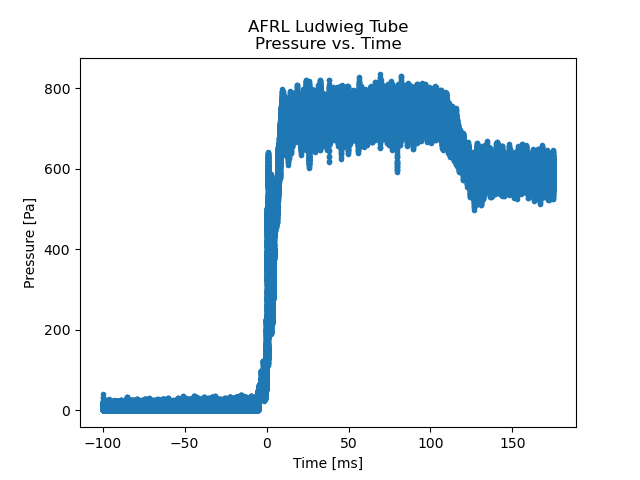
\includegraphics[scale=0.7]{pressure_vs_time}
				\label{Pressure_vs_Time}
				\caption{Pressure vs. Time in Test Section}
			\end{figure}

			\begin{figure}[h]
				\centering
				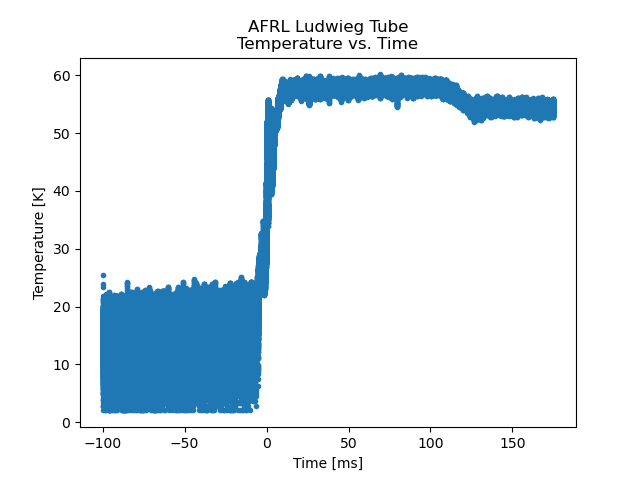
\includegraphics[scale=0.7]{temperature_vs_time}
				\label{Temperature_vs_Time}
				\caption{Temperature vs. Time in Test Section}
			\end{figure}

			\begin{figure}[h]
				\centering
				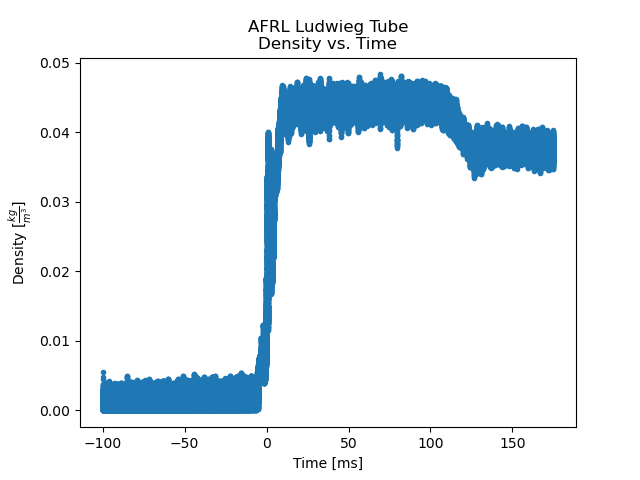
\includegraphics[scale=0.7]{density_vs_time}
				\label{Density_vs_Time}
				\caption{Density vs. Time in Test Section}
			\end{figure}
			\vspace{10in}
			
		\end{enumerate}
			\clearpage
			\item Generally useful wind-tunnel data is collected n the test section between $25 < t < 75 \  ms$. How "steady" is the pressure during that period (i.e., what is the standard deviation about the mean value during that time?
			\addcontentsline{toc}{subsection}{(c)}
		\begin{enumerate}[label=\arabic*.]
			\item{\textbf{Givens}}\\
			\addcontentsline{toc}{subsubsection}{Givens}
			$t = [25\,,75] \ \unit{ms}$
			\item{\textbf{Solution}}\\
			Using Python's \textit{statistics} module, the mean and standard deviation of the pressure measurements between $25 < t < 75 \ \unit{ms}$ are easily calculated:
			
			\begin{empheq}[box=\fbox]{align}
				\mu_{pressure} &= 729.27 \ \unit{Pa} \nonumber\\
				\sigma_{pressure} &= 23.56 \ \unit{Pa} \nonumber
			\end{empheq}

			\addcontentsline{toc}{subsubsection}{Solution}
		\end{enumerate}
			\item At $t=50 \ \unit{\milli\second}$, what is the entropy difference between the upstream and test-section air? Recall,
			\begin{equation*}
				s_2 - s_1 = c_p \ln(\frac{T_2}{T_1}) - R \ln(\frac{p_2}{p_1}) \,.
			\end{equation*}
			You may use $c_p = 1000 \ \unit{\joule/\kilogram.\kelvin}$ and $R = 287 \ \unit{\joule/\kilogram.\kelvin}$. Does this make sense? Why or why not?
			\addcontentsline{toc}{subsection}{(d)}
		\begin{enumerate}[label=\arabic*.]
			\item{\textbf{Givens}}\\
			$c_p = 1000 \ \unit{\joule/\kilogram.\kelvin}$\\
			$R = 287 \ \unit{\joule/\kilogram.\kelvin}$\\
			$T_1 = 500 \ K$\\
			$p_1 = 1380 \ \unit{kPa}$
			\addcontentsline{toc}{subsubsection}{Givens}

			\item{\textbf{Assumptions}}\\
			Assuming isentropic flow for purposes of solving relations to get all needed values. 
			\addcontentsline{toc}{subsubsection}{Assumptions}

			\item{\textbf{Solution}}\\
			Given the previously calculated time histories for temperature and density, in cojunction with the pressure time history in the dataset, conditions at $t = 50 \ \unit{ms}$ are identified:
			\begin{align*}
				p_{50  \unit{ms}} &= 766.99 \ \unit{Pa}\\
				T_{50  \unit{ms}} &= 58.74 \ K
			\end{align*}\
			
			Recalling the discussion of the first and second law for reversible processes highlighted in \nameref{Sec:Problem1}, we begin by expressing the first law for a reversible process in terms of internal energy and enthalpy.   
			By definition, for internal energy: 
			\begin{equation*}
				\dd e = \delta q_{reversible} - p\dd \nu
			\end{equation*}
			
			Expressing the first law in terms of enthalpy:

			\begin{align*}
				\dd h &= \dd e + p\dd \nu + \nu \dd p\\
				\dd h &= \delta q_{reversible} - p\dd \nu + p\dd \nu + \nu \dd p\\
				\dd h &= \delta q_{reversible} + \nu \dd p\\
			\end{align*}

			Now, we examine the second law for a reversible process:

			\begin{align*}
				\dd s &= \frac{\delta q_{reversible}}{T}\\
				\delta q_{reversible} &= T \dd s
			\end{align*}

			Substituting this equation into the previous relations for $\dd h \textrm{and} \dd e$ yields the following, known as \textit{Gibb's Equations}:

			\begin{empheq}[box=\fbox]{align}
				T \dd s &= \dd e + p \dd \nu \nonumber \\
				T \dd s &= \dd h - \nu \dd p \nonumber
			\end{empheq}
			
			\textit{Note: To this point, only reversible assumptions have been made.}\\

			By making the assumption that the working fluid is a TPG, we can substitute specific heat relationships into the above equations, and additionally use the ideal gas equation of state to recast the final term of each equation in terms of a variable and its differential operator.
			Finally, we divide through by $T$ to isolate $\dd s$.

			\begin{align*}
				\dd s &= c_\nu \frac{\dd T}{T} + R {\frac{\dd \nu}{\nu}}\\
				\dd s &= c_p \frac{\dd T}{T} - R {\frac{\dd p}{p}} 
			\end{align*}
			
			We now examine the topmost equation involving $c_\nu$. Dividing through by $\dd T$ and integrating the equation from state $1$ to state $2$ yields an expression for the change in entropy generated between two states of a reversible process of a TPG.

			\begin{align*}
				\dd s &= c_\nu \frac{\dd T}{T} + R{\frac{\dd \nu}{\nu}}\\
				\int_1^2 \dd s &= \int_1^2 c_\nu \frac{\dd T}{T} + \int_1^2 R{\frac{\dd \nu}{\nu}}\\
				s_2 - s_1 &= c_v \ln{\left(\frac{T_2}{T_1}\right)} + R \ln{\left(\frac{\nu_2}{\nu_1}\right)}
			\end{align*}

			Performing the same integration for the other Gibb's Equation yields the equation given in the problem statement:

			\begin{equation*}
				s_2 - s_1 = c_p \ln(\frac{T_2}{T_1}) - R \ln(\frac{p_2}{p_1}) \,.
			\end{equation*}

			Substituting known values into the given equation:
			\begin{equation*}
				s_2 - s_1 = 1000 \left[\frac{\unit{\joule}}{\unit{\kilogram}\cdot \unit{\kelvin}}\right] 
				\ln{\left(\frac{58.74 \ [\unit{\kelvin}]}{500 \ [\unit{\kelvin}]}\right)}
				- 287 \left[\frac{\unit{\joule}}{\unit{\kilogram}\cdot \unit{\kelvin}}\right] 
				\ln{\left(\frac{766.99 \ [\unit{\pascal}]}{1380000 \ [\unit{\pascal}]}\right)}
			\end{equation*}
			\begin{equation*}
				\boxed{s_2-s_1 = 9.64 \ \unit{\joule/\kilogram.\kelvin}}
			\end{equation*}
			This value of entropy change makes sense even in light of the isentropic assumption made during data analysis. 
			There is a positive, non-zero entropy change due to the presence of a boundary layer and dissipative effects in the flow. 
			In addition, transducer error can contribute to inaccuracies in flow measurements. 
			Despite not being fully isentropic according to this calculation, the change in entropy is very small and indicates that the isentropic assumption is not unreasonable.
			\addcontentsline{toc}{subsubsection}{Solution}
			
		\end{enumerate}

			\item What do the isentropic relations show happens to the temperature of the flow as it expands to Mach-6? Look up the liquefaction temperature of air. What is it in Kelvin? With
			this knowledge, why do you think the air accelerated through high-speed wind tunnels is
			heated before every test?\\
			With an upstream starting pressure of $p = 1380 \  \unit{\kilo\pascal}$, calculate the upstream starting temperature for which the air temperature in the test section is equal to the liquefaction temperature at $ t = 50 \ \unit{\milli\second}$.
			\addcontentsline{toc}{subsection}{(e)}
		\begin{enumerate}[label=\arabic*.]
			\item{\textbf{Givens}}\\
			$p_{init} = 1380 \ \unit{\kilo\pascal}$
			\addcontentsline{toc}{subsubsection}{Givens}
			
			\item{\textbf{Assumptions}}\\
			$T_{liquefaction} = 77 \ \unit{\kelvin}$\\
			$P_{50 \unit{\ms}} = 766.99 \ \unit{\pascal}$\\
			$\gamma = 1.4$
			\addcontentsline{toc}{subsubsection}{Assumptions}
			
			\item{\textbf{Discussion}}\\
			Isentropic relations indicate that the temperature of a flow \textit{expanding} to Mach 6 will decrease.
			Recall the relationship between temperature and density at any 2 points in an isentropic flow:
			\begin{equation*}
				\frac{T_2}{T_1} = {\left(\frac{\rho_2}{\rho_1}\right)}^{\gamma-1}
			\end{equation*}
			As $\rho$ decreases in an accelerating, expanding supersonic flow, $T$ will also drop, albeit not at a one-to-one rate. \\
			The liquefaction temperature of air is $T_{liquefaction} = 77 \ \unit{\kelvin}$ according to \url{http://www.edubilla.com/invention/liquefaction-of-air/}.
			With this in mind, it makes sense that heating could be required for the supply air in a high-speed wind tunnel, to avoid accidentally generating condensation or liquid air in the tunnel that could compromise data collection.

			\addcontentsline{toc}{subsubsection}{Discussion}

			\item{\textbf{Solution}}\\
			Recall the relationship between temperature and pressure at any two points in an isentropic flow:

			\begin{equation*}
				\frac{T_2}{T_1} = \left({\frac{P_2}{P_1}}\right)^{\frac{\gamma-1}{\gamma}}
			\end{equation*}

			Setting $T_2$ equal to $T_{liquefaction}$ and rearranging to solve for $T_{upstream}$:

			\begin{equation*}
				T_{upstream} = \frac{T_{liquefaction}}{\left({\frac{P_2}{P_1}}\right)^{\frac{\gamma-1}{\gamma}}}
			\end{equation*}

			Substituting in known values and solving:

			\begin{equation*}
				T_{upstream} = \frac{77 \ \left[\unit{\kelvin}\right]}{\left(\frac{1380000 \ [\unit{\pascal}]}{766.99 \ [\unit{\pascal}]}\right)^{\frac{1.4-1}{1.4}}}
			\end{equation*}
			\begin{equation*}
				\boxed{T_{upstream} = 655.41\  \unit{\kelvin}}
			\end{equation*}
			
			The result of this calculation, along with previously-solved-for temperature at $t = 50 \ \unit{\ms}$ indicates that the air in the test section is \textit{already below the temperature required for liquefaction}.
			The reason this calculation may still be valid is that the liquefaction temperature of $77 \ \unit{\kelvin}$ is specifically for air under atmospheric pressure. 
			The pressure in the tunnel test-section at  $t = 50 \ \unit{\ms}$ is substantially less than atmospheric pressure, making liquefaction unlikely under these conditions.
			To confirm the calculation of temperature for the air in the test section, we can utilize the form of the isentropic equations that relies on total/stagnation conditions.
			\begin{equation*}
				\frac{T_0}{T} = 1 + \frac{\gamma-1}{2}M^2
			\end{equation*}
			
			In the equation above, $T_0$ represents the \textit{total temperature} of the flow, or the temperature that the flow would achieve if it were isentropically brought to a halt.
			Because the upstream conditions are initially stagnant, we can assume that $T_{init} = 500 \ \unit{\kelvin}$ is equivalent to $T_0 = 500 \ \unit{\kelvin}$. 
			In addition, we assume that the tunnel data taken from the .xlsx spreadsheet corresponds with a Mach 6 condition. 
			With these assumptions and this equation, a notional static temperature, $T_{static}$, is calculated, representative of an isentropic flow with the given initial conditions expanding to exactly Mach 6.
			
			\begin{align*}
				T_{static} &= \frac{T_0}{1 + \frac{\gamma-1}{2}M^2}\\
				T_{static} &= \frac{500 \left[\unit{\kelvin}\right]}{1 + \frac{1.4-1}{2}(6)^2}\\
				T_{static} &= 60.97 \ \unit{\kelvin}
			\end{align*}

			This result compares well with the calculated temperature from the spreadsheet data, where $T_{50 \unit{\milli\second}} = 58.74 \ \unit{\kelvin}$.
			Despite initially appearing to be a miscalculation, the temperature calculated from the data is validated by its relative closeness to the exact Mach 6 isentropic temperature for the given initial conditions.
			\addcontentsline{toc}{subsubsection}{Solution}
			
		\end{enumerate}

			\item A wind tunnel is used to simulate a flight vehicle flying through stagnant air. The
			difference is clearly the reference frame. If a hypersonic boost-glide vehicle is flying at Mach-6 at an altitude of 40 km where the air temperature is $\approx$ 250 K, do you think the air liquefies as it travels over the vehicle? Explain your reasoning.
			\addcontentsline{toc}{subsection}{(f)}
		\begin{enumerate}[label=\arabic*.]
			\item{\textbf{Discussion}}\\
			% TODO: clean up this discussion
			 Air will not liquefy when traveling over a Mach 6 boost-glide vehicle despite the low ambient temperature. 
			 The main difference between the air in the Ludwieg tube and the freestream air going over the Mach 6 vehicle hinges on the stagnation conditions of the flow.
			 The air in the Ludwieg tube is initially stagnant, with no velocity, and has to go through an expansion to achieve the Mach 6 condition.
			 This expansion is what causes the massive pressure drop that can lead to liquefaction of the air in the tunnel. 
			 When a boost-glide vehicle is traveling at Mach 6, the freestream air surrounding the vehicle does not have to undergo such a massive expansion.
			 In fact, the air is rapidly compressed by the vehicle's motion, causing shockwaves and temperature and density \textit{spikes}. \\
			 The stagnation/total conditions of a flow are dependent on the reference frame used to define them. 
			 Wind tunnel experimentation can rarely kinematically match both the Reynolds and Mach numbers in a flow.
			 Depending on whether the vehicle is fixed in the reference frame or a volume of air is fixed, the total conditions of the flow can vary.
			 The disparity between achievable conditions in a wind tunnel and flight conditions largely hinges on the enthalpies achievable, which is why ground tests and computational modeling must work in conjunction.
			  
			\addcontentsline{toc}{subsubsection}{Discussion}
			
		\end{enumerate}
	\end{enumerate}

	\newpage
	
	\begin{appendices}
		\section{Problem 1 Python Code}
		\label{Problem1Python}
		\lstinputlisting[language=Python,lastline=27]{../python/homework_1.py}
		\newpage

		\section{Problem 3 Python Code}
		\label{Problem3Python}

		\lstinputlisting[language=Python,firstline=28]{../python/homework_1.py}
		\newpage
	\end{appendices}
	
	
	%\newpage
	%\appendix
	%\section{Python Code}
	%\lstinputlisting[language=Python]{Module1.py}
	
\end{document}